\chapter{Introducción}
\label{cap:capitulo1}
\setcounter{page}{1}

\section{La robótica }
\label{sec:La_robótica}

La robótica es una disciplina compleja que se conforma de distintas áreas y campos de la ciencia y la tecnología. Entre ellas, las más destacables serían la mecánica, la electrónica,  la informática, la ingeniería de control, la física y la \ac{IA}. Todas estas disciplinas se unen en una que pretende idear, diseñar y construir robots, Máquinas capaces de realizar de manera automática y preferiblemente autónoma una o un conjunto de tareas para las cuales esta ha sido designada \cite{wikipedia-de-robot}\\

\bigskip

\begin{figure}[h] 
    \centering
    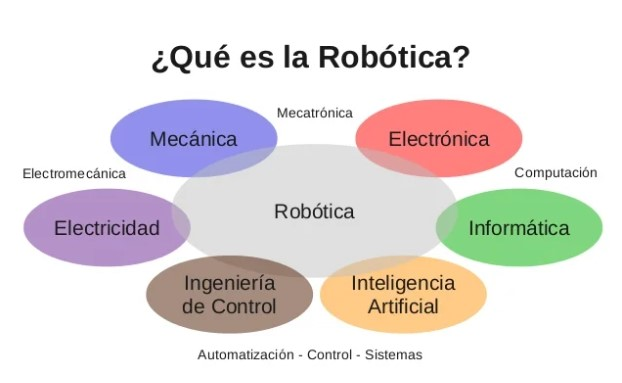
\includegraphics[width=0.7\linewidth]{imagenes/cap1/disciplinas_robotica.jpg} 
    \caption{Disciplinas que componen la robótica.}
    \label{fig:Disciplinas que componen la robótica.} 
\end{figure}

\bigskip

Con los recientes avances en mecatrónica, informática e \ac{IA}, la robótica ha encontrado su lugar en una amplia gama de sectores. En el sector industrial, los brazos robóticos desempeñan roles cruciales en cadenas de montaje, automatizando y refinando diversos procesos. Paralelamente, en el sector doméstico, la robótica ha transformado nuestras rutinas diarias: desde aspiradoras inteligentes que se desplazan con precisión por nuestros hogares, hasta avanzados robots de cocina que simplifican la preparación de alimentos.
\bigskip


\section{Los robots móviles }
\label{sec:Los_robots_móviles}

Los robots, a lo largo de su evolución, han sido clasificados de diversas maneras en función de su diseño, propósito y contexto de aplicación. Los robots humanoides, con su semejanza a la figura humana, buscan emular nuestros movimientos y comportamientos para adaptarse a nuestro mundo. Existen también robots colaborativos que, en lugar de reemplazar a los humanos, están diseñados para trabajar junto a nosotros en entornos compartidos. También podemos distinguir los ya mencionados robots industriales, sin embargo y a pesar de esta diversidad, existe una clasificación que destaca sobre el resto, debido a su gran importancia en la historia de la robótica y a su continuo desarrollo, estos son los robots móviles. Un robot móvil es un sistema robótico que puede desplazarse en distintos entornos y que cuenta con una serie de capacidades que le permiten ejecutar tareas complejas, ya sea de forma autónoma o controlados por un operador humano. \cite{los-robots-móviles}

\bigskip

\begin{figure}[h] 
    \centering
    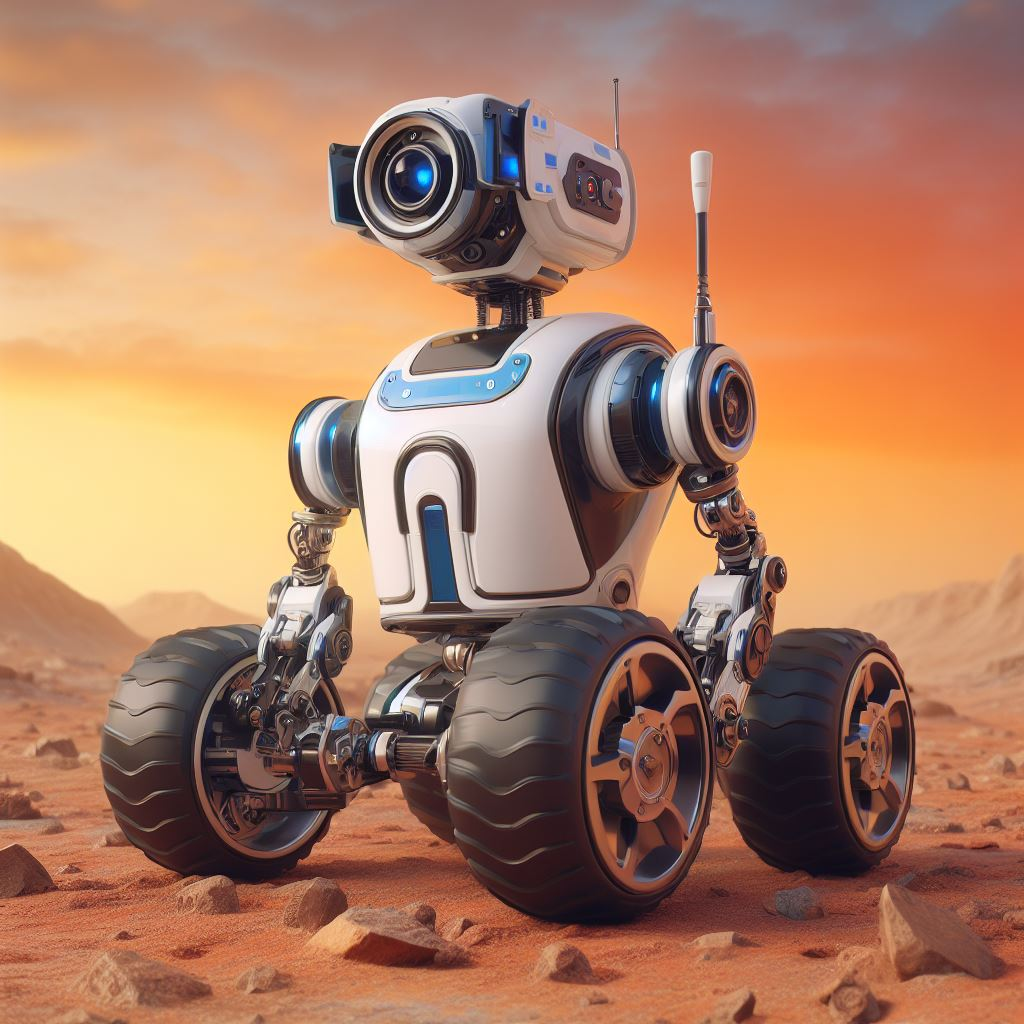
\includegraphics[width=0.7\linewidth]{imagenes/cap1/robot_movil.png} 
    \caption{Ilustración de un robot móvil generado por \acs{IA}.}
    \label{fig:Ilustración de un robot móvil generado por IA} 
\end{figure}

\bigskip

A diferencia de los robots fijos, que permanecen estacionarios y realizan tareas desde una posición establecida como por ejemplo los brazos roboticos en una cadena de montaje, los robots móviles \cite{robots-moviles-2} cuentan con la capacidad de desplazarse de un sitio a otro. Esto les otorga una libertad sin precedentes y les permite realizar todo tipo de acciones que para muchas otras máquinas resultan imposibles. Esta versatilidad se debe, en gran parte, a avanzados sistemas de sensores que les permiten percibir su entorno, algoritmos de navegación y control que delinean sus trayectorias; sistemas de comunicación que los conectan con otras máquinas, con bases de datos y teleoperadores e incluso con otros robots. Y a sofisticados actuadores, tales como ruedas, patas, hélices y un largo etcétera, en función de a qué medios deba adaptarse el robot.

\bigskip

En el panorama de la robótica móvil, a pesar de la diversidad y versatilidad de sus aplicaciones, una categoría ha destacado del resto. Los vehículos autónomos son, probablemente, los protagonistas de la robótica móvil del siglo XXI. Estos robots son vehículos equipados con sofisticados sensores que les permiten percibir su entorno, procesar esa información mediante algoritmos avanzados para reaccionar ante él de manera inteligente, imitando el comportamiento de conducción humano. Estos vehículos consiguen esta gran hazaña gracias a una característica muy importante: la conducción autónoma.

\bigskip

\section{La conducción autónoma }
\label{sec:La_conducción_autónoma}

La conducción, en su esencia, se refiere a la acción de guiar o controlar un vehículo, ya sea motorizado o no, con la finalidad de trasladarse de un lugar a otro. Desde tiempos prehistóricos, la humanidad ha tenido la necesidad de trasladarse y transportar bienes, materias primas y otras personas. esta necesidad impulsó la creación de vehículos sencillos como carros tirados por animales o vehículos impulsados por la propia potencia muscular del conductor, como las bicicletas.

\bigskip

Con el paso del tiempo y el avance de la ingeniería y la ciencia en el mundo de la automoción, en el siglo XIX aparecieron los primeros vehículos motorizados. Estos prototipos, movidos inicialmente por vapor y luego por combustibles fósiles, marcaron el inicio de una revolución en la movilidad y transformaron la manera en que las personas y mercancías se desplazaban. Sin embargo, estos vehículos requerían determinadas habilidades manuales y cognitivas por parte del conductor, además de amplios conocimientos de la máquina que se opera. Así, la conducción se convirtió en una habilidad que las personas debían estudiar, practicar y aprender. Adicionalmente, el acto de conducir, para ser ejecutado de manera correcta y segura, requiere de atención, calma y claridad mental, estados que en ocasiones resultan difíciles de mantener para los seres humanos, sobre todo en situaciones desconocidas, inciertas y estresantes, situaciones que son el pan de cada día de cualquier conductor. Todo esto ha hecho que la conducción sea una de las habilidades más difíciles de adquirir y a la vez más valoradas en la actualidad.

\bigskip

Debido a esto, la idea de vehículos que pudieran conducirse por sí mismos, sin necesidad de intervención humana y de las habilidades y atención del conductor, ha sido una aspiración de la humanidad por mucho tiempo, muy probablemente desde el inicio mismo de la conducción. Sin embargo, no fue hasta finales del siglo XX cuando esta idea empezó a parecer viable. Durante este período, la emergencia de la computación, la inteligencia artificial y una amplia gama de sensores avanzados resultaron en vehículos capaces de interpretar su entorno, tomar decisiones y operar sin intervención humana directa en ciertas condiciones estableciendo así el inició de la conducción autónoma. La conducción autónoma se define como la capacidad total o  parcial de que un vehículo pueda conducir autónomamente sin necesidad de un operador externo. \cite{la-conducción-autónoma}

\begin{figure}[h] 
    \centering
    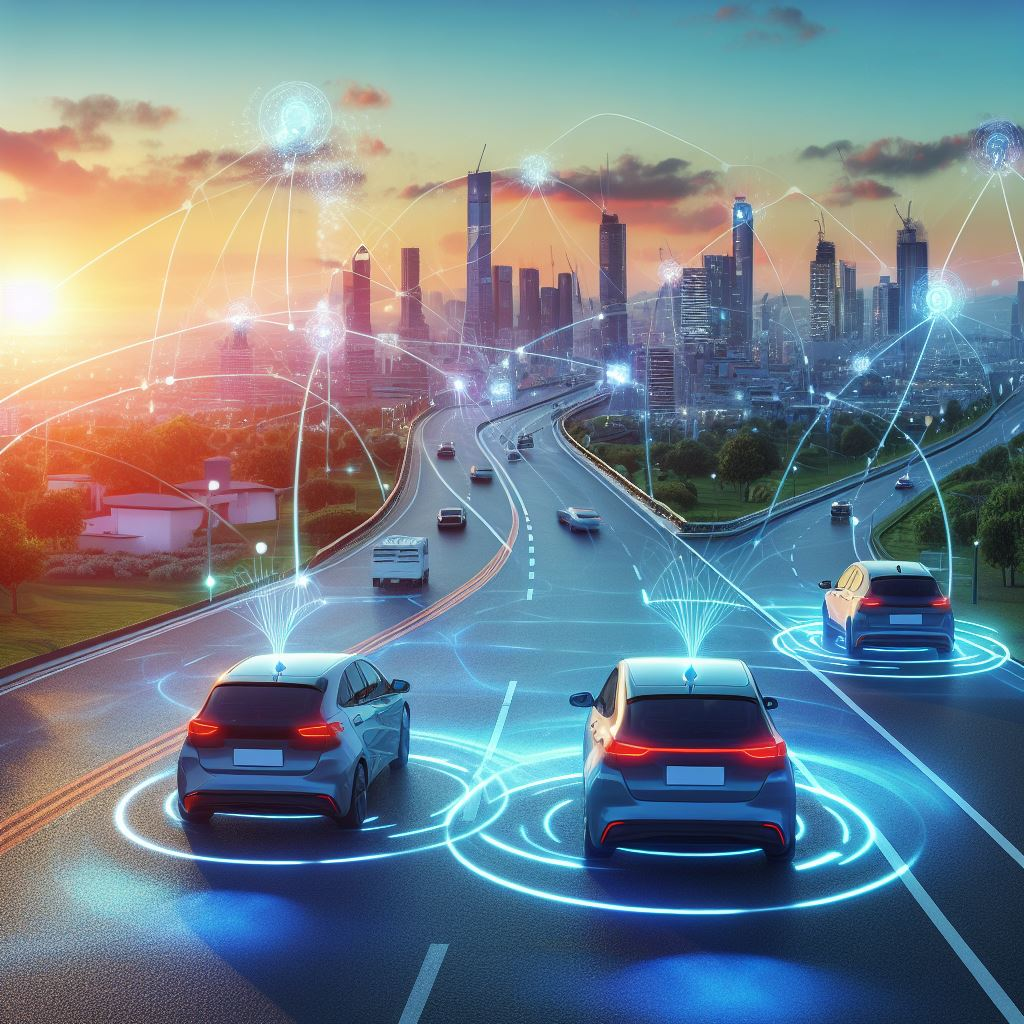
\includegraphics[width=0.7\linewidth]{imagenes/cap1/conduccion_autonoma.png} 
    \caption{Ilustración de coches autónomos generada por \ac{IA}.}
    \label{Ilustración de coches autónomos generada por IA}
\end{figure}


\newpage



Existen 6 niveles de conducción autónoma según el estándar establecido por la \ac{SAE} en el estándar J3016 \cite{estándar-j3016}

\begin{enumerate}
        \item \textbf{Nivel 0 (No Automation)}:
         El conductor humano es responsable de todas las tareas de conducción, incluso si el vehículo ofrece alguna intervención momentánea.
        \bigskip

    \item \textbf{Nivel 1 (Driver Assistance)}:

        El vehículo puede asistir al conductor en una única tarea de conducción (por ejemplo, control de crucero).
        El conductor sigue siendo responsable de la mayoría de las tareas y debe estar atento en todo momento.
       \bigskip

    \item \textbf{Nivel 2 (Partial Automation)}:

         El vehículo puede controlar simultáneamente dos tareas, como dirección y aceleración.
         A pesar de esta automatización, el conductor debe supervisar el sistema en todo momento.
       \bigskip

    \item \textbf{Nivel 3 (Conditional Automation)}:

         El vehículo puede realizar la mayoría de las tareas de conducción en ciertas condiciones, pero requerirá intervención humana cuando el sistema lo solicite.
         El conductor debe estar disponible para tomar el control, pero no necesita tener las manos en el volante todo el tiempo.
       \bigskip

    \item \textbf{Nivel 4 (High Automation)}:

        En ciertos escenarios o zonas geográficas específicas, el vehículo puede manejar todas las tareas de conducción.
        Fuera de estas zonas, el vehículo podría requerir que el conductor tome el control.
      \bigskip

    \item \textbf{Nivel 5 (Full Automation)}:

        El vehículo es completamente autónomo en todos los escenarios y condiciones.
        No necesita un volante, pedales ni un conductor humano.
      \bigskip
\end{enumerate}

\newpage

\begin{figure}[h] 
    \centering
    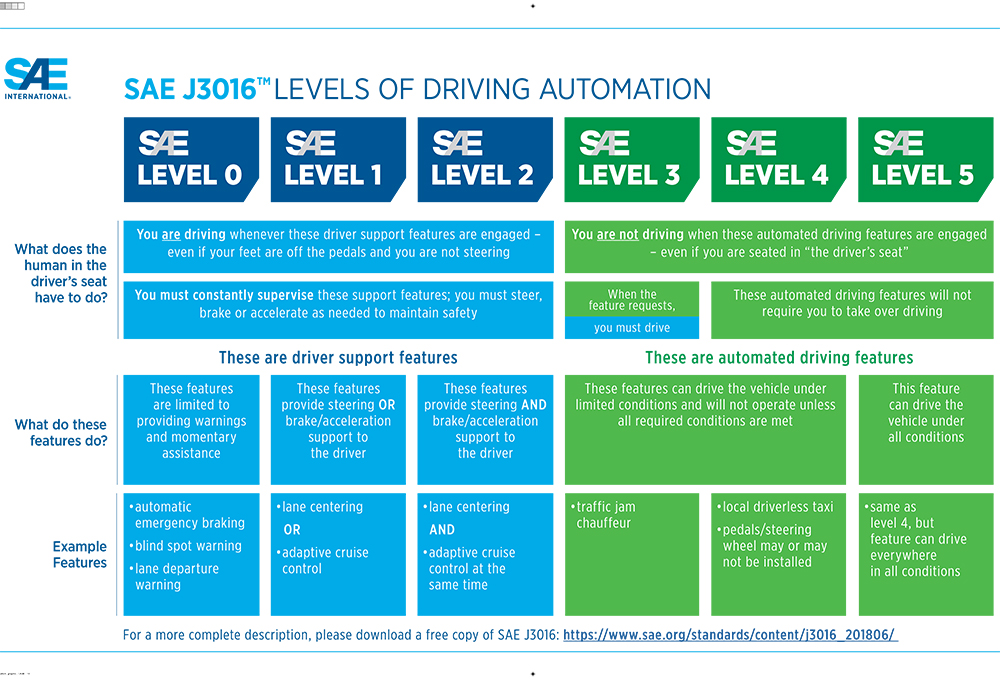
\includegraphics[width=1\linewidth]{imagenes/cap1/niveles_conduccion_autonoma.jpg} 
    \caption{Niveles de conducción autónoma según el estándar J3016}
    \label{fig:Niveles de conducción autónoma según el estándar J3016} 
\end{figure}

\bigskip

El final del siglo XX y el comienzo del siglo XXI marcaron una era significativa en el avance de la conducción autónoma. Los primeros sistemas y algoritmos para la conducción autónoma derivaban de los \ac{ADAS}. Según la página oficial de la DGT \cite{ADAS_DGT} estos sistemas representan un conjunto de tecnologías integradas en vehículos que no solo mejoran la seguridad sino también la experiencia del conductor. Operan con diferentes grados de autonomía y pueden influir en múltiples funciones del vehículo, como frenado, aceleración, dirección y señalización. Sistemas como el \ac{ISA}, que regula constantemente la velocidad del vehículo; el \ac{REV}, que alerta sobre obstáculos al retroceder; y el \ac{LKA}, que asegura que el vehículo permanezca dentro de un carril, sitúan a los coches que los incorporan dentro de los primeros 2 niveles de autonomía \cite{articulo-academico-tesla}. No obstante, con el auge de la \ac{IA}, la emergencia de las redes neuronales y los avances en computación, los sistemas \ac{ADAS} han evolucionado con rapidez. Este progreso ha permitido a empresas como Tesla desarrollar los primeros vehículos comerciales de nivel 2. En cuanto a los niveles de autonomía más avanzados tenemos a compañías como Waymo, quien como se explica en ese artículo académico \cite{tesla_y_robotaxi} esta embarcado en un proyecto para crear una flota de taxis autónomos.

\newpage

\begin{figure}[h] 
    \centering
    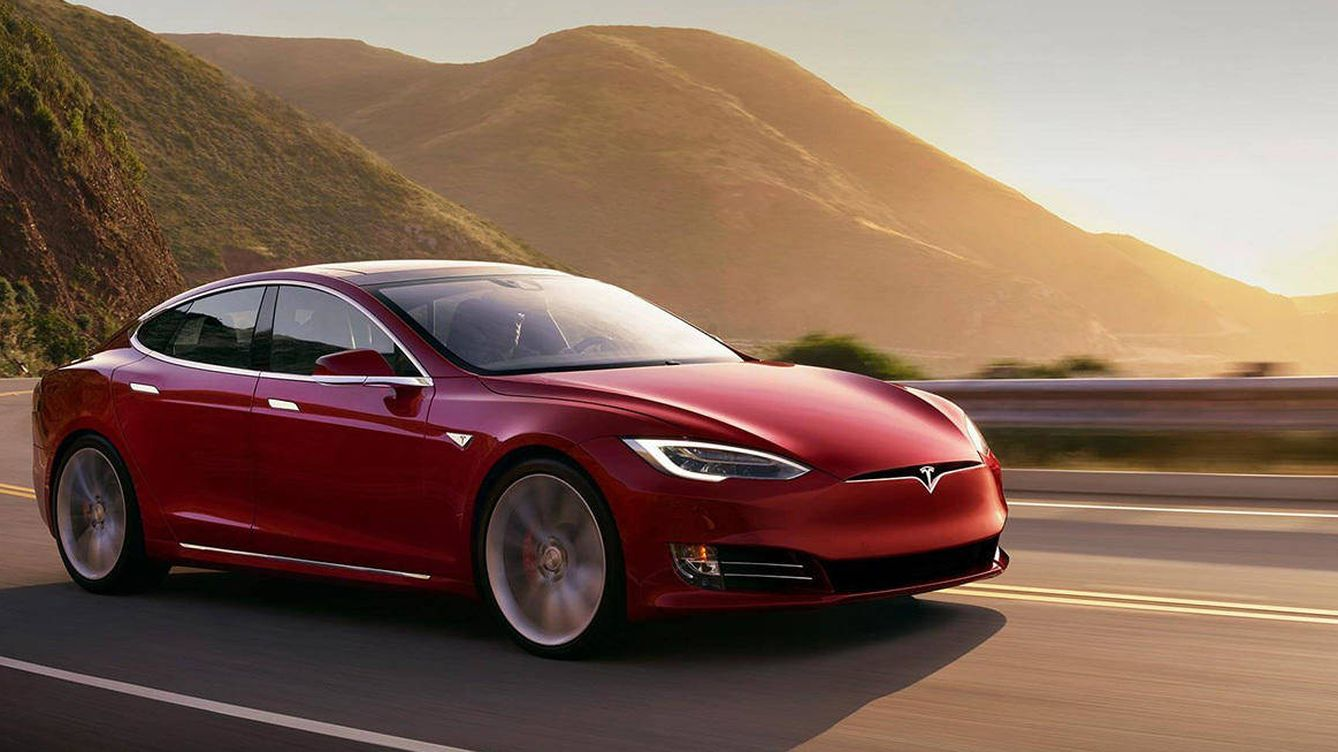
\includegraphics[width=0.7\linewidth]{imagenes/cap1/tesla.jpg} 
    \caption{Vehículo tesla}
    \label{fig:Vehículo tesla} 
\end{figure}


\bigskip

Los llamados robotaxis  \cite{robotaxi} , son actualmente una serie de taxis de nivel de autonomía 4 que operan en algunas ciudades de Estados Unidos. Estos vehículos están pensados para transportar pasajeros de manera completamente autónoma, sin la necesidad de un conductor humano, de hecho estos taxis futuristas no incluyen pedales ni volante como se puede observar en la figura \ref{fig:robotaxi}. Los robotaxi actualmente realizan viajes con pasajeros reales seleccionados en algunas zonas de Phoenix y San Francisco con el fin de recopilar datos y en general probar y madurar esta nueva tecnología para así en un futuro próximo convertir los robotaxis en un producto comercial que revolucione el transporte en las ciudades

\bigskip

\begin{figure}[h] 
    \centering
    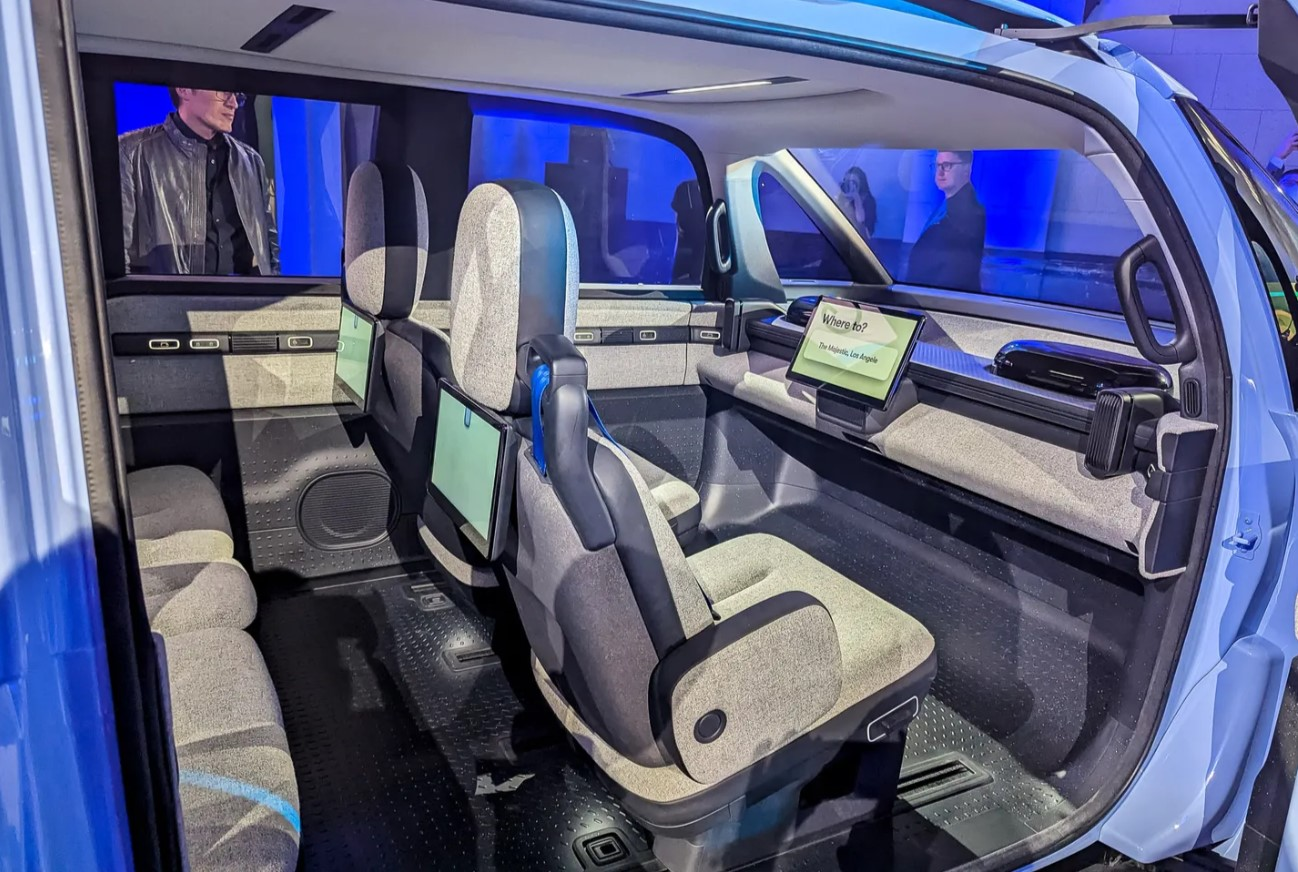
\includegraphics[width=0.7\linewidth]{imagenes/cap1/waymo_robotaxi.jpg} 
    \caption{Interior de un robotaxi de Waymo}
    \label{fig:robotaxi}
\end{figure}


\newpage

Sin embargo, a pesar de todos los avances de los últimos años en el ámbito de la conducción autónoma, esta problemática sigue sin estar completamente solucionada y los vehículos de nivel 4 y 5 de autonomía todavía son solo prototipos y no productos comerciales certificados y testados como podemos leer en este \ac{TFM} \cite{estado_del_arte_conducción_autónoma}. Esto se debe a que la conducción autónoma es una de las áreas más desafiantes dentro de la ingeniería y la robótica, dada la inmensa complejidad y variabilidad de los escenarios en los que estos vehículos deben operar. Estos entornos no son estáticos, sino que están en constante cambio y movimiento. Carreteras en constante transformación, condiciones meteorológicas cambiantes, variaciones de luz, obstáculos inesperados y una amplia variedad de usuarios de la vía, desde peatones hasta ciclistas y otros vehículos, hacen que la carretera sea uno de los entornos más impredecibles. Añadiendo una capa adicional de complejidad, se encuentra el factor humano. No solo los vehículos autónomos deben anticipar y responder a las acciones de los conductores humanos, que pueden ser a menudo ilógicas o imprevistas, sino que además deben garantizar la máxima seguridad para los peatones y otros usuarios de la vía. Convivir en un espacio compartido con seres humanos requiere de un cuidado y precisión extraordinarios, pues el más mínimo error podría tener consecuencias extremadamente graves como se menciona en este artículo académico en la revista Nature \cite{peligros_conducción_autónoma}

\bigskip

No obstante, una conducción autónoma perfecta promete revolucionar radicalmente el paradigma de movilidad y seguridad en nuestras carreteras tal y como explica este artículo publicado en la revista ScienceDirect \cite{la_revolución_de_la_conducción_autónoma}. La mayoría de los accidentes en la carretera son causados por errores humanos, ya sea por distracción, fatiga o decisiones erróneas en situaciones críticas. Los vehículos autónomos, operando con una combinación de sensores avanzados y algoritmos sofisticados, tienen el potencial de minimizar estos errores, reaccionando más rápidamente y de manera más precisa que un humano ante situaciones imprevistas. Además, los sistemas de conducción autónoma podrían gestionar de forma más eficiente el flujo de tráfico. Al poder comunicarse entre sí, los vehículos podrían coordinarse para evitar atascos, optimizar el uso de carriles y reducir las congestiones, resultando en viajes más rápidos y eficientes para todos. Por último, pero no menos importante, liberar a los humanos de la tarea de conducir abre un mundo de posibilidades. Las personas podríamos ocupar todo el tiempo que dedicamos hoy en día a la conducción en otras acciones más provechosas o entretenidas: leer, ver una película, trabajar o incluso descansar. Esto mejoraría la calidad de vida al proporcionar tiempo adicional para actividades personales o productivas. En definitiva, las ventajas que nos presenta la conducción autónoma son múltiples y muy interesantes; es una tecnología que, sin duda, cambiará el mundo.

\section{La inteligencia artificial en la conducción autónoma}
\label{sec:La inteligencia artificial en la conducción autónoma}

La \ac{IA} ha desempeñado un papel fundamental en la evolución de la conducción autónoma, permitiendo que los vehículos interpreten su entorno, tomen decisiones y se adapten a situaciones cambiantes. Al principio, la \ac{IA} en la conducción autónoma se basaba en algoritmos más básicos basados en visión artificial y procesamiento de imágenes. Sin embargo, pronto se hizo evidente que para alcanzar los niveles más altos de autonomía era necesario un enfoque más sofisticado para gestionar la complejidad. Esto condujo a la adopción y desarrollo de técnicas más avanzadas.

\textbf{Las redes neuronales} se han convertido en herramientas esenciales en el campo de la conducción autónoma \cite{Implementación_de_redes_neuronales_para_conducción_autónoma}. Estas redes, que imitan la estructura y el funcionamiento de las neuronas humanas, son particularmente aptas para tareas como la detección y la identificación de objetos. Al ser entrenadas con grandes cantidades de datos, pueden reconocer patrones y categorizar objetos en tiempo real con una precisión impresionante como se muestra en el siguiente \ac{TFG} de un estudiante de la universidad de \ac{ULPGC} \cite{detección_de_objetos_con_redes_neuronales}

\textbf{El imitation learning}, o aprendizaje por imitación \cite{imitation-learning-2}, es una técnica que permite a los sistemas de \ac{IA} aprender a partir de la observación directa de acciones realizadas por humanos u otros agentes. En el contexto de la conducción autónoma, se puede utilizar para enseñar a los vehículos a imitar las decisiones y acciones de conductores humanos experimentados en diversas situaciones, permitiendo que los vehículos aprendan comportamientos más naturales. En el \ac{TFM} que a continuación se cita se explora una solución para la conducción autónoma basada en imitation learning \cite{conducción_autónoma_imitation_learning}.

\textbf{El aprendizaje por refuerzo} es otra técnica de \ac{IA} crucial en la conducción autónoma. Este método entrena modelos de \ac{IA} a través de recompensas y penalizaciones, permitiéndoles aprender a tomar decisiones óptimas en situaciones específicas \cite{RL-2}. Por ejemplo, un vehículo autónomo podría ser recompensado por evitar obstáculos y penalizado por acercarse demasiado a ellos, aprendiendo con el tiempo a navegar de manera más segura y eficiente. En la documentación de continuación se puede encontrar información más detallada sobre el aprendizaje por refuerzo \cite{aprendizaje_por_refuerzo}

\newpage

\begin{figure}[h]
	\centering
	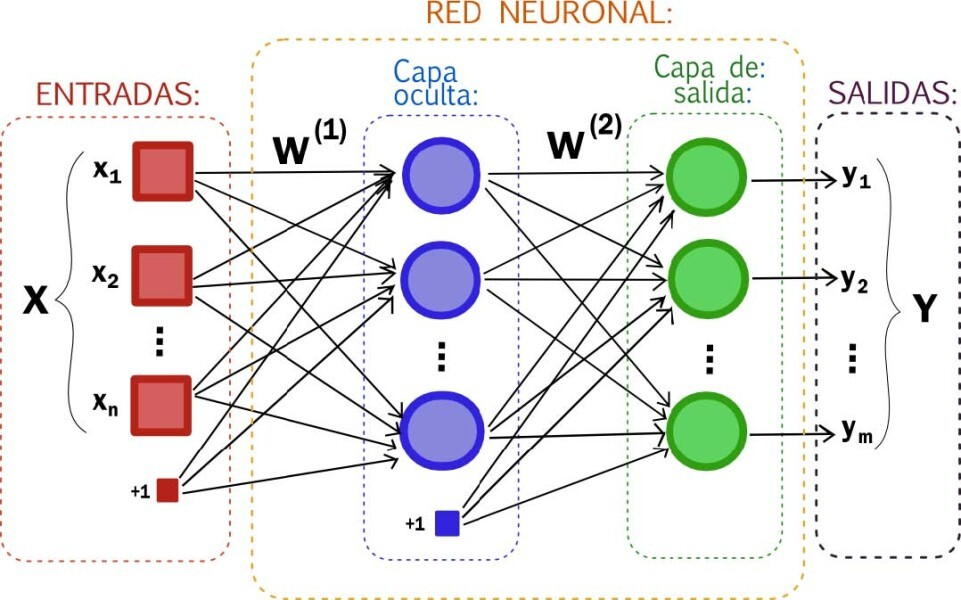
\includegraphics[width=0.7\linewidth]{imagenes/cap1/red_neuronal.jpeg}
	\caption{Ilustración de una red neuronal}
	\label{fig:Ilustración de una red neuronal}
\end{figure}

En resumen, la inteligencia artificial ha revolucionado significativamente el ámbito de la conducción autónoma. Las principales empresas tecnológicas y automotrices, como Waymo, Tesla y Cruise, han desarrollado y probado vehículos con niveles avanzados de autonomía, principalmente en niveles 2 y 3 e incluso en algunos casos con capacidades limitadas de nivel 4 en entornos específicos. A pesar de los logros técnicos, la complejidad que representa navegar por nuestras carreteras sitúa aún lejos vehículos capaces de alcanzar niveles 4 y 5 completos de autonomía \cite{Niveles-altos-autonomía}.

\section{ Conducción autónoma en CARLA con adaptación al tráfico basado en aprendizaje por refuerzo}
\label{sec:Conducción autónoma en CARLA basada en aprendizaje por refuerzo con adaptación al tráfico}

El \ac{TFG} que a continuación se presenta aborda una investigación académica sobre la conducción autónoma basada en aprendizaje por refuerzo. Se pretende solucionar varias problemáticas relacionadas con el seguimiento de carril con un vehículo autónomo de manera fluida y segura. Por otro lado, aparte de esta hazaña este \ac{TFG} pretende llegar un paso mas allá diseñando sistemas de seguimiento de carril con funciones añadidas como la capacidad de frenar para evitar la colisión frontal con obstáculos y adaptarse al tráfico presente en la vía de manera fluida.

\bigskip




  